\documentclass[11pt,a4paper]{ivoa}
\input tthdefs
\input gitmeta

\title{Authentication for Non-Browser Clients in the VO}

% see ivoatexDoc for what group names to use here; use \ivoagroup[IG] for
% interest groups.
\ivoagroup{Distributed Services \& Protocols}

\author{Patrick Dowler}
\author{Mark Taylor}
\author{Sara Bertocco}

\editor{Sara Bertocco}

% \previousversion[????URL????]{????Concise Document Label????}
\previousversion{This is the first public release}


\begin{document}
\begin{abstract}
Some, though not all, services in the Virtual Observatory are
restricted to users who have been authenticated and are authorized to use them.
This situation is far from unique to the VO,
and there is much industry-standard technology to manage authentication.
However, it largely assumes that authenticating clients,
often browser-based, understand how authentication is to be done
for a particular service.
This document addresses a problem apparently not covered
by existing standards, namely how a VO client can discover
authentication requirements and use the corresponding mechanisms
to supply user credentials
when pointed at a compliant VO service, without requiring out-of-band
information.
\end{abstract}


\section*{Acknowledgments}

\textcolor{red}{Editor's note: this section has to be
updated/rewritten. Authors who have someone to thank should
add here acknowledgments}
This document derives from discussions among the Grid and Web Services
working-group of IVOA. It is particularly informed by prototypes built
by Mark Taylor (University of Bristol) and Patrick Dowler
(Canadian Astronomy Data Centre).


\section*{Conformance-related definitions}

The words ``MUST'', ``SHALL'', ``SHOULD'', ``MAY'', ``RECOMMENDED'', and
``OPTIONAL'' (in upper or lower case) used in this document are to be
interpreted as described in IETF standard RFC2119 \citep{std:RFC2119}.

The \emph{Virtual Observatory (VO)} is a
general term for a collection of federated resources that can be used
to conduct astronomical research, education, and outreach.
The \href{https://www.ivoa.net}{International
Virtual Observatory Alliance (IVOA)} is a global
collaboration of separately funded projects to develop standards and
infrastructure that enable VO applications.


\section{Introduction}

???? Write something ????

\subsection{Role within the VO Architecture}

\begin{figure}
\centering

% As of ivoatex 1.2, the architecture diagram is generated by ivoatex in
% SVG; copy ivoatex/archdiag-full.xml to role_diagram.xml and throw out
% all lines not relevant to your standard.
% Notes don't generally need this.  If you don't copy role_diagram.xml,
% you must remove role_diagram.pdf from SOURCES in the Makefile.

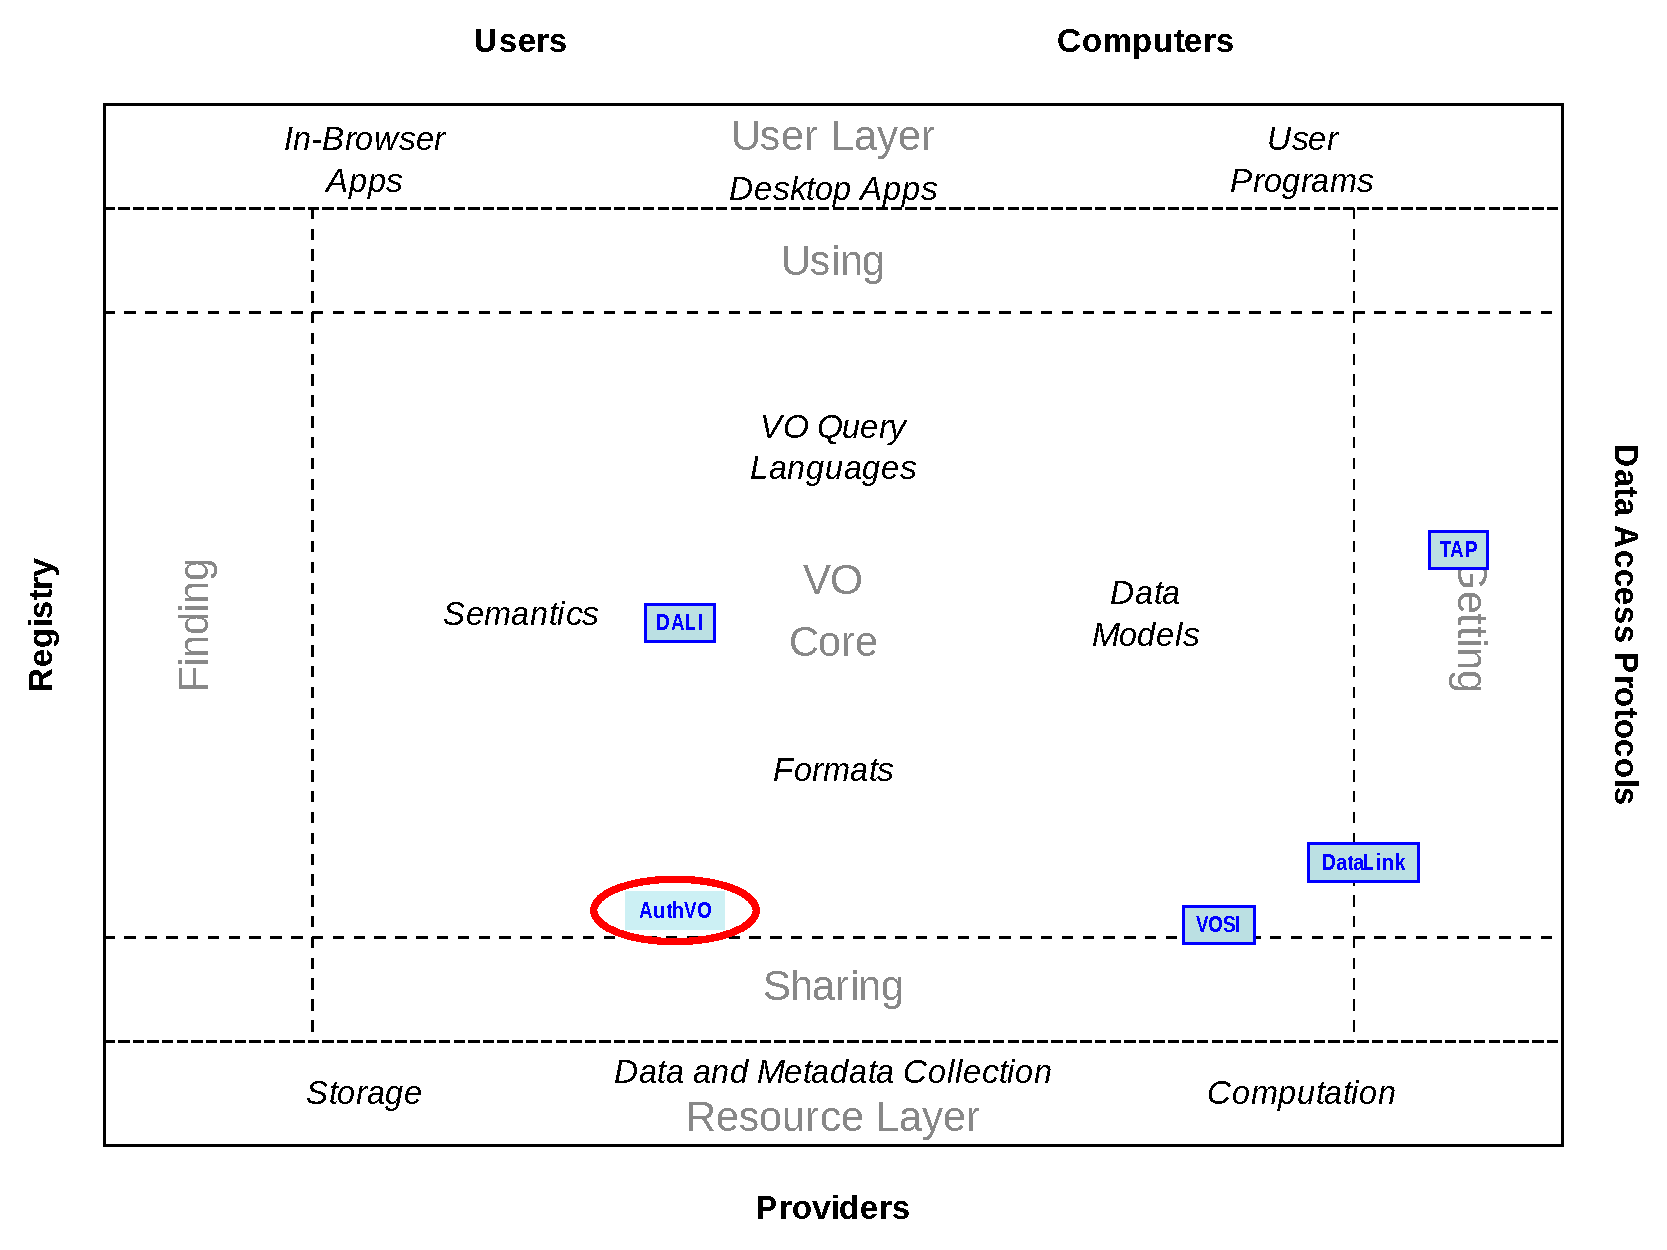
\includegraphics[width=0.9\textwidth]{role_diagram.pdf}
\caption{Architecture diagram for this document}
\label{fig:archdiag}
\end{figure}

Fig.~\ref{fig:archdiag} shows the role this document plays within the
IVOA architecture \citep{2021ivoa.spec.1101D}.

???? and so on, LaTeX as you know and love it. ????

\appendix
\section{Changes from Previous Versions}

No previous versions yet.
% these would be subsections "Changes from v. WD-..."
% Use itemize environments.


% NOTE: IVOA recommendations must be cited from docrepo rather than ivoabib
% (REC entries there are for legacy documents only)
\bibliography{ivoatex/ivoabib,ivoatex/docrepo}


\end{document}
